Die früheren Kapitels beschreiben mittels Objektendiagramms die Struktur der Anwendungen nach dem Starten.

    Die Schichten sind mittels \textbf{\nameref{DependencyInjection}} miteinander verknüpft.

    Beispiel für \textbf{Port}-\textbf{Adapter}-\textbf{Controller} Verbindung:

    \begin{figure}[H]
        \centering
        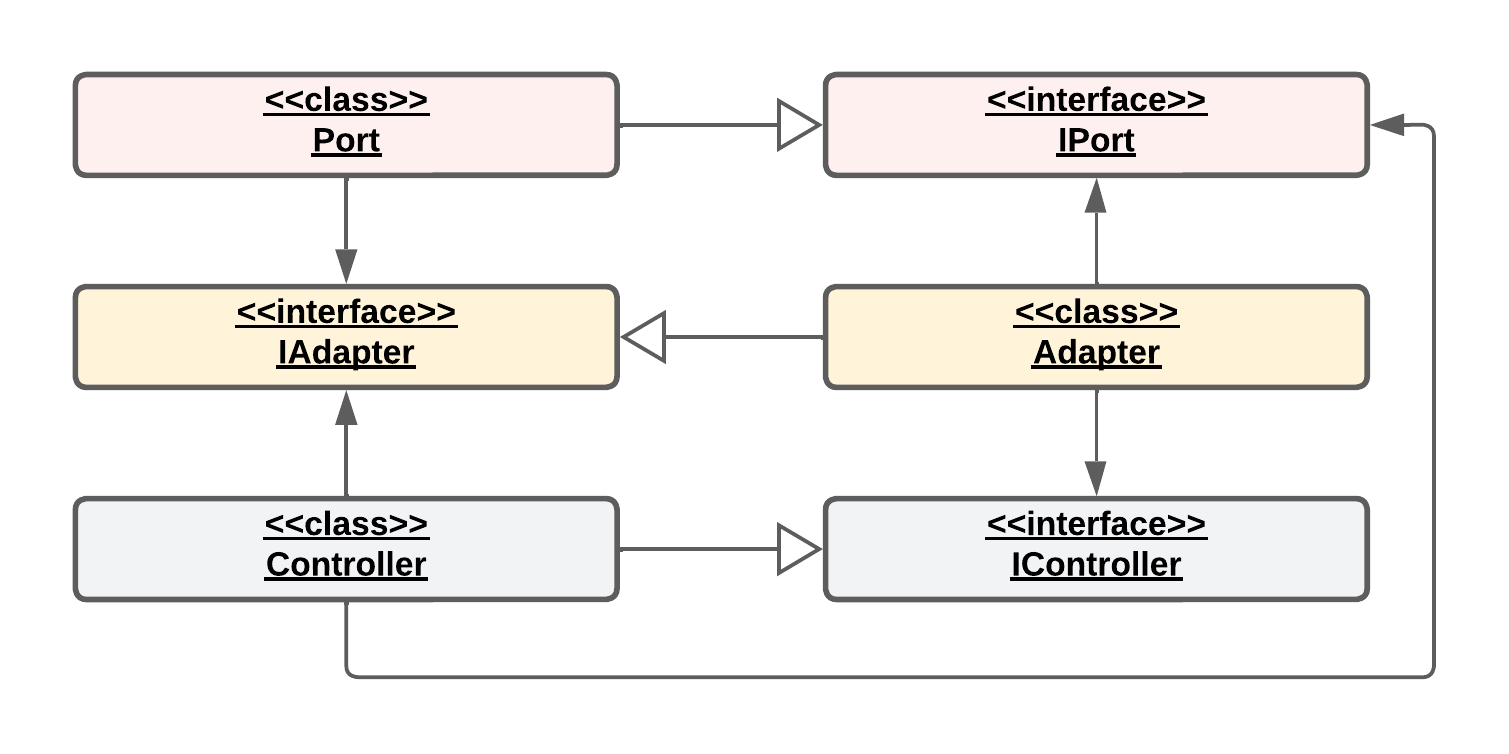
\includegraphics[width=12cm]{./images/Klassendiagramm Port-Adapter.png}
        \caption[Klassendiagramm Port-Adapter-Controller]{Klassendiagramm Port-Adapter-Controller \footnotemark}
        \label{fig:FullCDPAC}
    \end{figure}
    \footnotetext{Eigene Quelle}

    Im Klassendiagramm \ref{fig:FullCDPAC} sind alle Klassen miteinander über ein Interface verbunden.
    Dies ermöglicht leichte und schnelle Ersetzbarkeit der Schichten und 
    somit lässt sich jeder Zustand der Umgebung um einer Schicht simulieren. 
    Das ist Voraussetzung für Testbarkeit jeder einzelnen Schicht unabhängig von den anderen Schichten.